% Diagrama de atividades do agendamento. Gera AtividadeAgendamentoo.png.
\documentclass[border=8pt]{standalone}
\usepackage[utf8]{inputenc}
\usepackage[T1]{fontenc}
\usepackage{tikz}
\usetikzlibrary{shapes.geometric,positioning,arrows.meta,calc}
\tikzset{
  acao/.style={rectangle, rounded corners=5pt, draw, text width=5.6cm, align=center,
    minimum height=0.85cm, inner sep=4pt},
  decisao/.style={diamond, aspect=3.4, draw, text width=4.1cm, align=center, inner sep=-1pt},
  inicio/.style={circle, fill=black, minimum size=0.5cm, inner sep=0pt},
  fim/.style={circle, draw, double, double distance=1.2pt, fill=black, minimum size=0.45cm, inner sep=0pt},
  seta/.style={-{Latex[length=2.2mm]}},
  rot/.style={font=\small},
}
\begin{document}
\hyphenpenalty=10000\exhyphenpenalty=10000
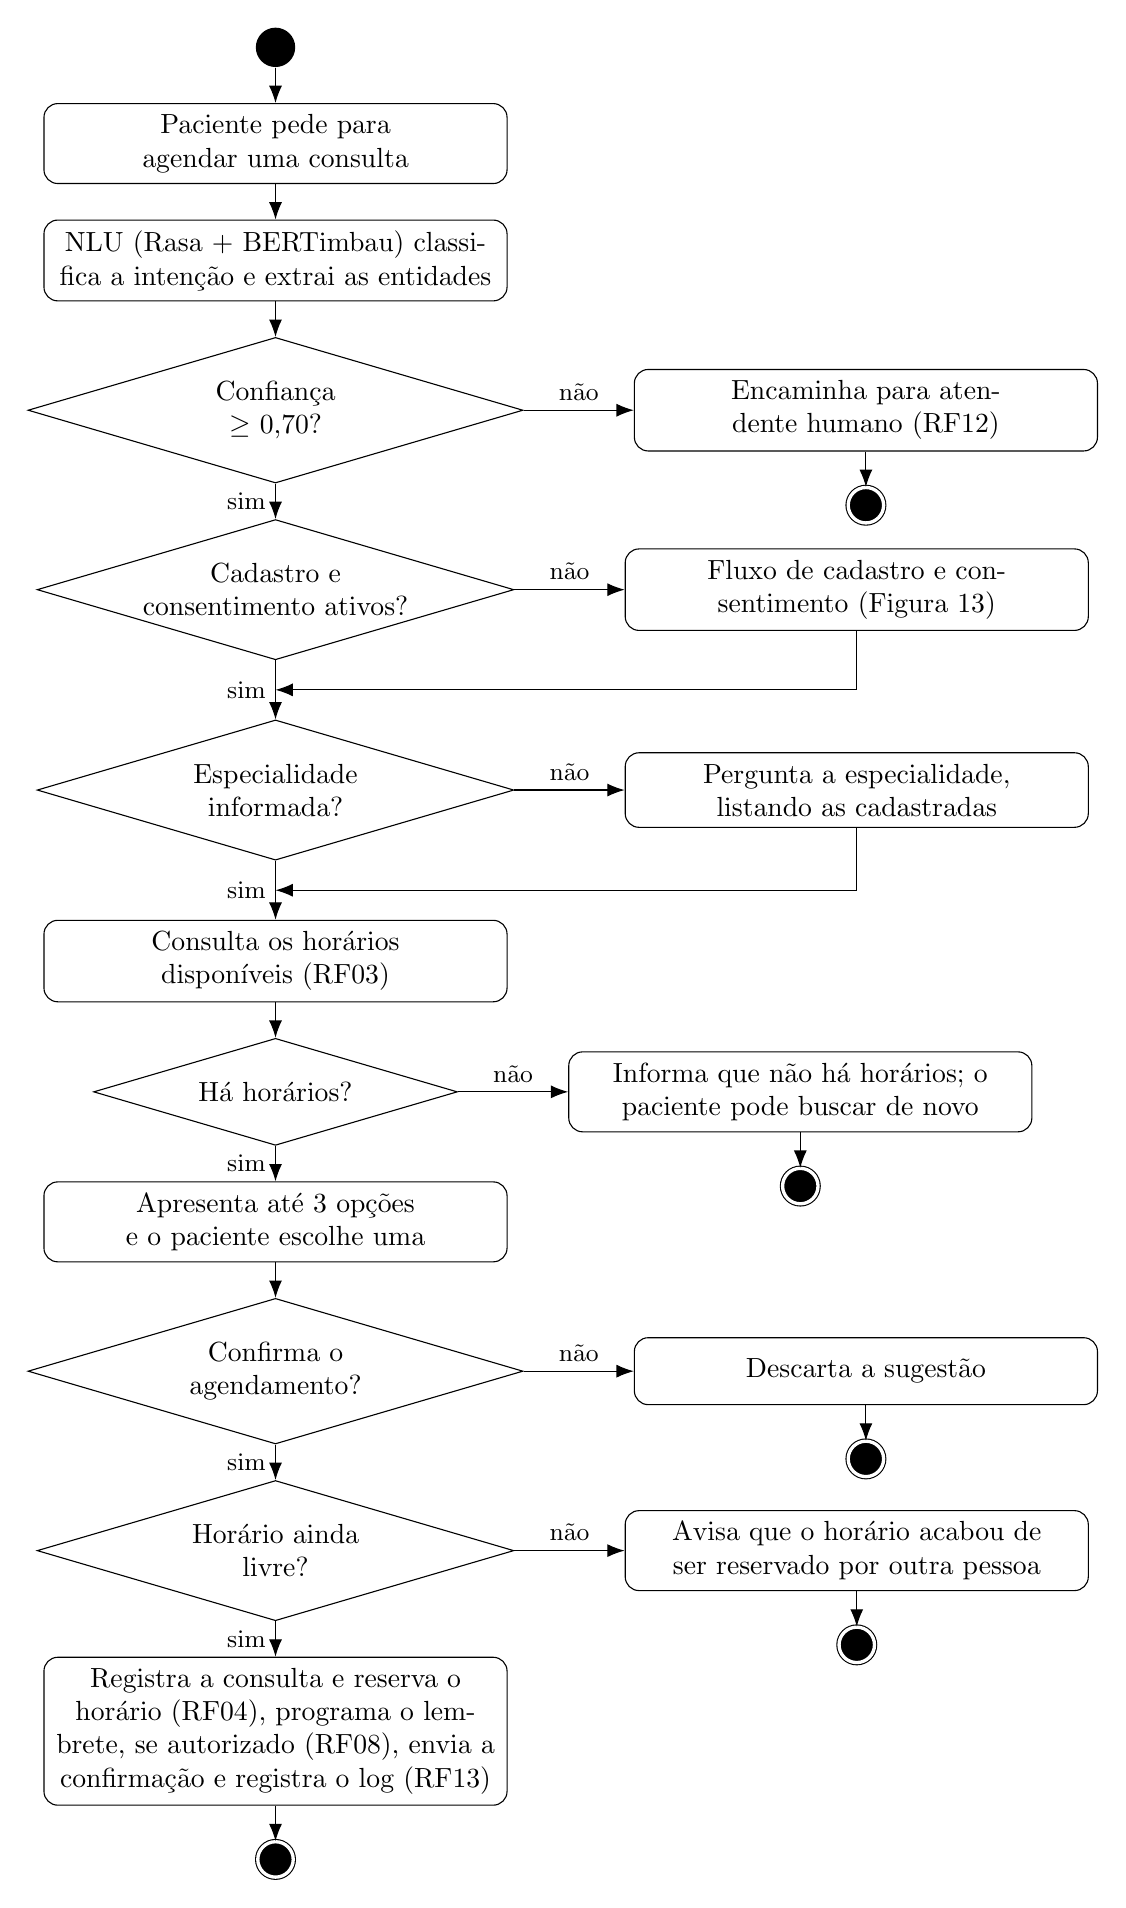
\begin{tikzpicture}[node distance=0.45cm and 1.4cm]
\node[inicio] (ini) {};
\node[acao, below=of ini] (pede) {Paciente pede para agendar uma consulta};
\node[acao, below=of pede] (nlu) {NLU (Rasa + BERTimbau) classifica a intenção e extrai as entidades};
\node[decisao, below=of nlu] (conf) {Confiança \\ $\geq$ 0,70?};
\node[acao, right=of conf] (humano) {Encaminha para atendente humano (RF12)};
\node[fim, below=of humano] (f1) {};

\node[decisao, below=of conf] (cad) {Cadastro e \\ consentimento ativos?};
\node[acao, right=of cad] (fluxocad) {Fluxo de cadastro e consentimento (Figura 13)};

\node[decisao, below=0.75cm of cad] (esp) {Especialidade \\ informada?};
\node[acao, right=of esp] (pergunta) {Pergunta a especialidade, listando as cadastradas};

\node[acao, below=0.75cm of esp] (busca) {Consulta os horários disponíveis (RF03)};
\node[decisao, below=of busca] (ha) {Há horários?};
\node[acao, right=of ha] (semhor) {Informa que não há horários; o paciente pode buscar de novo};
\node[fim, below=of semhor] (f2) {};

\node[acao, below=of ha] (opcoes) {Apresenta até 3 opções e o paciente escolhe uma};
\node[decisao, below=of opcoes] (confirma) {Confirma o \\ agendamento?};
\node[acao, right=of confirma] (descarta) {Descarta a sugestão};
\node[fim, below=of descarta] (f3) {};

\node[decisao, below=of confirma] (livre) {Horário ainda \\ livre?};
\node[acao, right=of livre] (tomado) {Avisa que o horário acabou de ser reservado por outra pessoa};
\node[fim, below=of tomado] (f4) {};

\node[acao, below=of livre] (fim) {Registra a consulta e reserva o horário (RF04), programa o lembrete, se autorizado (RF08), envia a confirmação e registra o log (RF13)};
\node[fim, below=of fim] (f5) {};

\draw[seta] (ini) -- (pede);
\draw[seta] (pede) -- (nlu);
\draw[seta] (nlu) -- (conf);
\draw[seta] (conf) -- node[rot,above]{não} (humano);
\draw[seta] (humano) -- (f1);
\draw[seta] (conf) -- node[rot,left]{sim} (cad);
\draw[seta] (cad) -- node[rot,above]{não} (fluxocad);
\draw[seta] (fluxocad.south) |- ($(cad.south)!0.5!(esp.north)$);
\draw[seta] (cad) -- node[rot,left]{sim} (esp);
\draw[seta] (esp) -- node[rot,above]{não} (pergunta);
\draw[seta] (pergunta.south) |- ($(esp.south)!0.5!(busca.north)$);
\draw[seta] (esp) -- node[rot,left]{sim} (busca);
\draw[seta] (busca) -- (ha);
\draw[seta] (ha) -- node[rot,above]{não} (semhor);
\draw[seta] (semhor) -- (f2);
\draw[seta] (ha) -- node[rot,left]{sim} (opcoes);
\draw[seta] (opcoes) -- (confirma);
\draw[seta] (confirma) -- node[rot,above]{não} (descarta);
\draw[seta] (descarta) -- (f3);
\draw[seta] (confirma) -- node[rot,left]{sim} (livre);
\draw[seta] (livre) -- node[rot,above]{não} (tomado);
\draw[seta] (tomado) -- (f4);
\draw[seta] (livre) -- node[rot,left]{sim} (fim);
\draw[seta] (fim) -- (f5);
\end{tikzpicture}
\end{document}
